\documentclass[conference]{IEEEtran}
\IEEEoverridecommandlockouts
\usepackage{cite}
\usepackage{amsmath,amssymb,amsfonts}
\usepackage{graphicx}
\usepackage{booktabs}
\usepackage{url}
\usepackage{textcomp}
\usepackage{xcolor}
\def\BibTeX{{\rm B\kern-.05em{\sc i\kern-.025em b}\kern-.08em
    T\kern-.1667em\lower.7ex\hbox{E}\kern-.125emX}}

\graphicspath{{models/}}
\begin{document}

\title{Chess2FEN: Converting Chessboard Photographs to FEN with Homography and CNN Classification}

\author{\IEEEauthorblockN{Your Name}
\IEEEauthorblockA{\textit{Your Department} \\
\textit{Your University/Organization}\\
City, Country \\
your.email@example.com}
}

\maketitle

\begin{abstract}
Chess2FEN is a minimal computer vision pipeline that converts a photograph of a chessboard into Forsyth--Edwards Notation (FEN). The system uses manual corner annotation to compute a homography, warps the board to a canonical top-down view, splits the image into 64 square crops, and applies a convolutional neural network (CNN) classifier to predict one of 13 classes (empty plus 12 chess pieces). The predicted piece grid is converted to a FEN piece-placement string. Evaluated on 234 labeled board photographs (15 unique positions) with per-image corner annotations, the model achieves 87.18\% square-level accuracy and 2.14\% exact piece-placement match, with an average inference time of 0.97 s per board on a CPU-only environment.
\end{abstract}

\begin{IEEEkeywords}
chessboard recognition, FEN, homography, OpenCV, TensorFlow, MobileNetV2, image classification
\end{IEEEkeywords}

\section{Introduction}
Converting chessboard images into a machine-readable representation is useful for digitizing over-the-board games, building analysis tools, and enabling human--computer interaction. Forsyth--Edwards Notation (FEN) compactly represents a board position and is widely used by chess engines and databases.

Chess2FEN targets a practical setting: a phone photo of a physical board under uncontrolled lighting and perspective. Rather than attempting end-to-end detection of all pieces and squares in the raw image, the pipeline first normalizes viewpoint via homography, then performs piece classification on per-square crops. This design simplifies learning and makes intermediate outputs interpretable for debugging.

\section{Related Work}
Prior chessboard recognition systems typically combine geometric normalization with either template matching or machine-learned classification. Modern approaches often use convolutional neural networks for piece recognition and employ keypoint/corner detection for board localization. Chess2FEN follows this classical decomposition but emphasizes simplicity, reproducibility, and a small code footprint.

\section{Methodology}
\subsection{Corner Annotation and Board Warping}
Given an input image, four board corners are annotated in chess order (a8, h8, h1, a1). A planar homography is then computed to warp the board into an $800\times800$ top-down view using a perspective transform. This establishes a fixed coordinate system where a8 is the top-left corner.

\subsection{Square Extraction}
The warped board image is split into an $8\times8$ grid. Each square is cropped with padding (10 px by default) to reduce border artifacts and neighboring-piece bleed. The resulting 64 crops are resized to $96\times96$ pixels and normalized to $[0,1]$.

\subsection{Piece Labeling and FEN Encoding}
For dataset construction, each board photo is paired with a known FEN piece-placement string. The FEN is expanded into 64 labels (in a8-to-h1 order) and used to label the extracted crops. During inference, the predicted labels are converted back into a FEN piece-placement string by collapsing runs of empty squares per rank.

\subsection{Classifier Architecture}
The classifier uses transfer learning with MobileNetV2 as a frozen feature extractor and a small dense head (global average pooling, dropout, and two dense layers with softmax output). The label space has 13 classes: \texttt{empty} and the 12 piece types (white/black $\times$ king, queen, rook, bishop, knight, pawn).

\section{Experimental Setup}
\subsection{Data}
The repository contains 234 chessboard photographs organized into 15 position folders under \texttt{input\_imgs/}. Each folder includes a \texttt{fen.txt} and \texttt{fen\_list.csv} mapping image filenames to the corresponding FEN piece placement, and a matching corner annotation JSON in \texttt{data/corners/}. The dataset generation step produces 64 labeled crops per photograph.

\subsection{Metrics}
Two metrics are reported:
\begin{itemize}
\item \textbf{Square accuracy}: fraction of correctly classified squares across all evaluated boards.
\item \textbf{Exact placement accuracy}: fraction of boards for which the entire predicted FEN piece-placement string matches the ground-truth placement exactly.
\end{itemize}

\subsection{Implementation}
The pipeline is implemented in Python using OpenCV for geometric transforms and TensorFlow/Keras for inference and training. The inference entry point loads \texttt{models/classifier.keras} and its class ordering from \texttt{models/classifier.classes.json}.

\section{Results and Discussion}
Table~\ref{tab:metrics} summarizes evaluation on all 234 labeled images in the repository. While square-level accuracy is relatively high, exact-board accuracy is low because a single square mistake makes the full placement incorrect. The most frequent confusions involve pawns and empty squares, consistent with small, low-texture regions and similar silhouettes in cropped images.

\begin{table}[htbp]
\caption{Evaluation metrics on 234 labeled board photographs}
\begin{center}
\begin{tabular}{l r}
\toprule
Metric & Value \\
\midrule
Boards evaluated & 234 \\
Squares evaluated & 14{,}976 \\
Square accuracy & 87.18\% \\
Exact piece-placement accuracy & 2.14\% \\
Average runtime (CPU) & 0.97 s/board \\
\bottomrule
\end{tabular}
\label{tab:metrics}
\end{center}
\end{table}

\begin{figure}[htbp]
\centerline{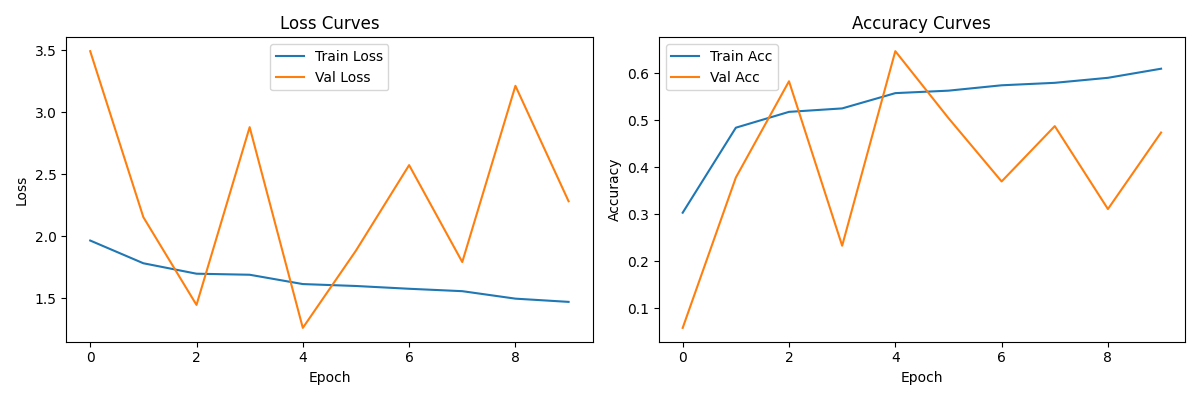
\includegraphics[width=\linewidth]{classifier.curves.png}}
\caption{Training curves saved by the training script.}
\label{fig:curves}
\end{figure}

\begin{figure}[htbp]
\centerline{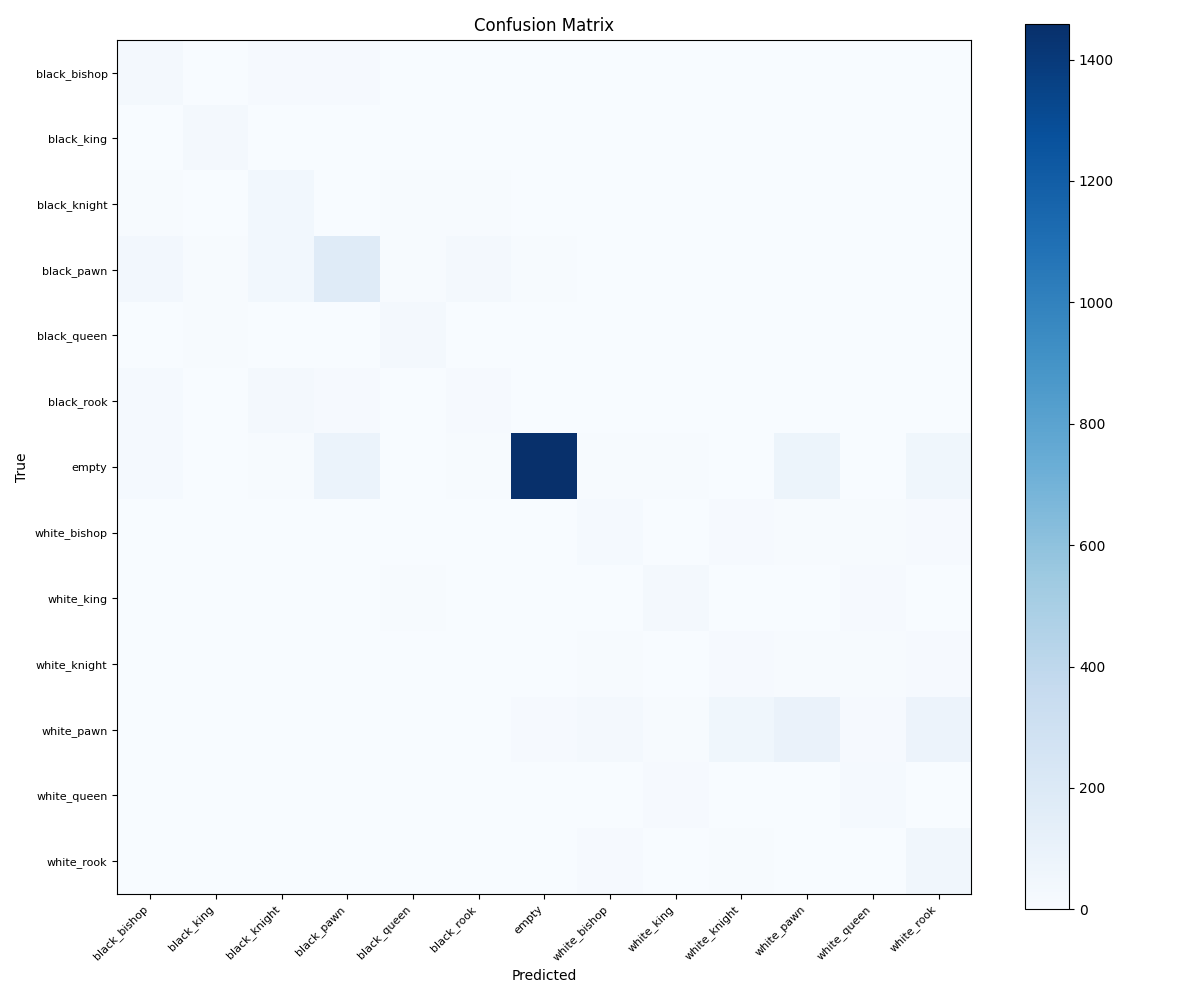
\includegraphics[width=\linewidth]{classifier.confusion.png}}
\caption{Confusion matrix saved by the training script.}
\label{fig:conf}
\end{figure}

\subsection{Limitations}
The current system requires manual corner annotation, which limits scalability and is sensitive to user error. The approach also assumes a fully visible board and does not model occlusions (hands, glare) or enforce chess legality constraints during decoding. Additionally, a still image cannot reliably infer dynamic FEN fields such as castling rights and en passant targets; the implementation therefore emits only the piece placement and fills remaining fields with defaults.

\section{Conclusion and Future Work}
Chess2FEN demonstrates an interpretable and compact pipeline for mapping chessboard photos to FEN using homography normalization and CNN-based square classification. Future work includes automatic board corner detection, data collection across different boards and piece sets for improved generalization, and structured decoding that incorporates chess rules (e.g., legality constraints) to improve full-board accuracy. Extending the system to video with temporal smoothing and occlusion handling is another promising direction.

\section*{References}

\begin{thebibliography}{00}
\bibitem{b1} G. Bradski, ``The OpenCV Library,'' \textit{Dr. Dobb's Journal of Software Tools}, 2000.
\bibitem{b2} M. Abadi \textit{et al.}, ``TensorFlow: a system for large-scale machine learning,'' in \textit{Proc. 12th USENIX Symp. Operating Systems Design and Implementation (OSDI)}, 2016, pp. 265--283.
\bibitem{b3} M. Sandler, A. Howard, M. Zhu, A. Zhmoginov, and L.-C. Chen, ``MobileNetV2: Inverted residuals and linear bottlenecks,'' in \textit{Proc. IEEE Conf. Computer Vision and Pattern Recognition (CVPR)}, 2018, pp. 4510--4520.
\bibitem{b4} R. Hartley and A. Zisserman, \textit{Multiple View Geometry in Computer Vision}, 2nd ed. Cambridge, U.K.: Cambridge Univ. Press, 2003.
\bibitem{b5} N. Fiekas, ``python-chess: a chess library for Python,'' 2012--2025. [Online]. Available: \url{https://python-chess.readthedocs.io/}
\bibitem{b6} Chess Programming Wiki, ``Forsyth--Edwards Notation (FEN),'' accessed Dec. 2025. [Online]. Available: \url{https://www.chessprogramming.org/Forsyth-Edwards_Notation}
\end{thebibliography}

\end{document}
